\documentclass{chi-ext}
\copyrightinfo{ }

\title{Duo-Portal, a HTML5 cooperative game}

\numberofauthors{2}
\author{
  \alignauthor{
  	\textbf{Frederico Schardong}\\
  	\affaddr{University of Calgary}\\
  	\affaddr{Calgary, CA T2N 1N4 Canada}\\
  	\email{fschardo@ucalgary.ca}
  }\alignauthor{
  	\textbf{Cédric Guillot}\\
  	\affaddr{University of Calgary}\\
  	\affaddr{Calgary, CA T2N 1N4 Canada}\\
  	\email{cedricson@ucalgary.ca}
  }
}

% Paper metadata (use plain text, for PDF inclusion and later re-using, if desired)
\def\plaintitle{Duo-Portal, a HTML5 cooperative game}
\def\plainauthor{Frederico Schardong}
\def\plainkeywords{Cooperative, HTML5, online game, portal}
\def\plaingeneralterms{Cooperative, HTML5, online game, portal}

\hypersetup{
  % Your metadata go here
  pdftitle={\plaintitle},
  pdfauthor={\plainauthor},  
  pdfkeywords={\plainkeywords},
  pdfsubject={\plaingeneralterms},
  % Quick access to color overriding:
  citecolor=black,
  linkcolor=blue,
  menucolor=black,
  urlcolor=blue,
}

\usepackage{graphicx}   % for EPS use the graphics package instead
\usepackage{balance}    % useful for balancing the last columns
\usepackage{bibspacing} % save vertical space in references

\begin{document}

\maketitle

\begin{abstract}
In this paper we describe the implementation of a cooperative online game in HTML5 inspired from the successful game Portal by Valve.
\end{abstract}

\category{H.5.m}{Information interfaces and presentation (e.g., HCI)}{Miscellaneous}

\terms{\plaingeneralterms}

\section{Introduction}
In this project we are going to implement a 2D casual version of Portal game created by Valve in a platform style (side view) for two players. The game will require the players to cooperate to reach each level’s goal and consequently proceed to the next level. The only way to reach each level’s goal is having both players cooperating. The game can be played online in a web browser.\\

\begin{figure}
\hspace*{-0.4\columnwidth}% displace figure
\parbox{1.4\columnwidth}{
  \centering
  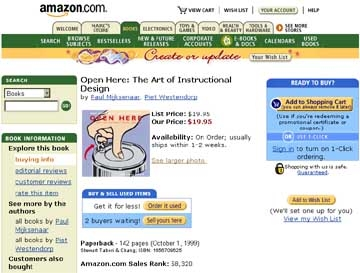
\includegraphics[width=1.4\columnwidth]{sample.jpg}
  \caption{Insert a caption below each figure. Images can "float" around body text, like this example.}
  \label{fig:sample}
}
\end{figure}

\section{Design principles}
We decided to rely on Crafty, a HTML5 game engine in order to code the game. The players first need to connect to the server hosting the game. Then, they are shown a list of players that they can play with. After inviting a player, the game is starting.\\
The players are immersed on the playing platform and have to reach the exit door in order to proceed to the next level. To do so, each of them has a portal and those 2 portals must be combined in order to go further into the level. What stands between the players and the exit door is a set of two kinds of walls. The "white" walls allow players to set their portal on it while the "black" walls do not allow it. This type of wall adds difficulty to the levels by forcing the players to think more carefully where they want to set their portals.\\
We designed the game to be casual. Consequently:\\
\begin{itemize}
\item The gameplay is very simple: you just need to use common commands to move around the game space.
\item The games do not last more than a couple of minutes (and most of the time, they will only last for 30 seconds).
\item Anybody can play these games as they are very simple. The fun of it comes from the communication between players but not from the complexity of the game.
\item You just need to launch a web browser, connect to the web site, invite a friend, and you are playing!
\end{itemize}

\subsection{Manual user}
This manual user can also be found on the login page so that they know what commands to use ingame.
\begin{itemize}
\item Use right and left arrow for walking in a direction.
\item Space for jumping.
\item Right click for opening your portal on "white" walls ("black" walls cannot be targeted).
\end{itemize}

\section{Implementation Details}


\section{Design Evolution}
\subsection{During the game coding}


\subsection{Designing the levels}
Once the game was operational, we started to work on the level design. We easily came up with 3 levels, but once they were implemented, finding new interesting designs of our own was pretty difficult. We came to understand that coding a game and actually implementing an interesting user experience are two very distinct areas. That is why we decided to stick with 3 levels as a good start for further work on the game.

\section{Discussion and Conclusion}

\balance
\bibliographystyle{acm-sigchi}
\bibliography{sample}

\end{document}